%====================================================================
\section{AlphaFold2 : principe général}
%====================================================================

\paragraph{Le problème.} La séquence d'acides aminés d'une protéine détermine sa structure tridimensionnelle~\cite{anfinsen1973}, mais le nombre de conformations possibles est tel qu'une exploration exhaustive est impossible. On appelle cela le \og problème du repliement \fg{}~\cite{ebi_course}. Plutôt que de simuler le repliement physique, AlphaFold2~\cite{jumper2021} \emph{apprend}, à partir des structures connues de la PDB, la relation entre séquence et structure.

\paragraph{Entrée et sortie.} L'utilisateur fournit uniquement la \textbf{séquence} de la protéine (format FASTA). AlphaFold2 renvoie les \textbf{coordonnées 3D} de tous les atomes lourds (fichier PDB ou mmCIF), accompagnées de \textbf{mesures de confiance}.

\paragraph{Le MSA et la coévolution.} La première étape consiste à rechercher, dans de grandes bases de séquences, des protéines \emph{homologues} (issues d'un ancêtre commun) et à les aligner : c'est l'\textbf{alignement multiple de séquences} (MSA). Chaque ligne est une séquence homologue et chaque colonne une position équivalente de la protéine. Le MSA apporte deux informations structurales :
\begin{itemize}
  \item la \textbf{conservation} : une position qui ne varie jamais est probablement essentielle (cœur hydrophobe, site actif) ;
  \item la \textbf{coévolution} : si deux résidus sont en contact, une mutation de l'un est souvent compensée par une mutation de l'autre, sinon la protéine perd sa structure. Deux colonnes qui varient \emph{ensemble} indiquent donc deux résidus probablement proches dans l'espace~\cite{ebi_course}.
\end{itemize}
Plus le MSA est profond et diversifié, plus ces signaux sont fiables. À l'inverse, une protéine \og orpheline \fg{}, sans homologues, est en général mal prédite.

\paragraph{Les grandes étapes.} La figure~\ref{fig:schema} résume le processus :
\begin{enumerate}
  \item \textbf{Recherche d'homologues} dans les bases de séquences (MSA) et, en option, de structures connues similaires (\emph{gabarits}) ;
  \item \textbf{Evoformer} : un réseau de neurones fait circuler l'information entre le MSA et une \og représentation de paires \fg{}, qui décrit pour chaque couple de résidus $(i,j)$ leur relation spatiale probable ;
  \item \textbf{Module de structure} : il transforme la représentation de paires en coordonnées 3D (squelette, puis chaînes latérales) ;
  \item \textbf{Recyclage} : la structure obtenue est réinjectée dans le réseau (3 fois par défaut) pour l'affiner.
\end{enumerate}

\paragraph{Pourquoi des mesures de confiance ?} Une prédiction n'est pas une mesure expérimentale : sa qualité varie d'une protéine à l'autre, et même d'une région à l'autre. AlphaFold2 a été entraîné à \emph{estimer sa propre erreur}. Il produit un score local par résidu, le \textbf{pLDDT}, et une erreur relative entre paires de résidus, la \textbf{PAE} (section~\ref{sec:analyse}). Sans ces scores, l'utilisateur ne pourrait pas distinguer une région fiable d'une région inventée.

\begin{figure}[H]
  \centering
  \resizebox{\textwidth}{!}{% Schéma personnel du fonctionnement général d'AlphaFold2
\begin{tikzpicture}[
  font=\small,
  node distance=6mm and 8mm,
  data/.style={draw, rounded corners=2pt, fill=blue!8, align=center, minimum height=10mm, text width=26mm},
  proc/.style={draw, thick, fill=orange!15, align=center, minimum height=12mm, text width=32mm},
  outp/.style={draw, rounded corners=2pt, fill=green!12, align=center, minimum height=10mm, text width=30mm},
  db/.style={draw, cylinder, shape border rotate=90, aspect=0.2, fill=gray!15, align=center, text width=20mm, minimum height=12mm},
  arr/.style={-{Stealth[length=2.5mm]}, thick},
  lab/.style={font=\scriptsize\itshape, align=center}
]
  % Entrée
  \node[data] (seq) {\textbf{Séquence}\\\texttt{MADQLTEEQ...}\\(FASTA)};

  % Recherche d'homologues
  \node[db, above right=2mm and 10mm of seq] (dbseq) {Bases de\\séquences\\(UniRef, env.)};
  \node[db, below right=2mm and 10mm of seq] (dbpdb) {Gabarits\\(PDB)\\\scriptsize optionnel};

  % Représentations
  \node[data, right=38mm of seq, yshift=9mm] (msa) {\textbf{MSA}\\séquences homologues\\alignées};
  \node[data, right=38mm of seq, yshift=-9mm] (pair) {\textbf{Représentation\\de paires} (i,j)};

  % Réseau
  \node[proc, right=of msa, yshift=-9mm] (evo) {\textbf{Evoformer}\\échange d'information\\MSA $\leftrightarrow$ paires};
  \node[proc, right=of evo] (sm) {\textbf{Module de\\structure}\\coordonnées 3D};

  % Sorties
  \node[outp, below=12mm of sm] (pdb) {\textbf{Structure 3D}\\(PDB / mmCIF)};
  \node[outp, left=of pdb] (conf) {\textbf{Confiance}\\pLDDT (par résidu)\\PAE (par paire)};

  % Flèches
  \draw[arr] (seq) -- (dbseq) node[lab, midway, above left]{recherche\\(MMseqs2)};
  \draw[arr] (seq) -- (dbpdb);
  \draw[arr] (dbseq) -- (msa);
  \draw[arr] (dbpdb.east) -- (pair.west);
  \draw[arr] (msa.east) -- (evo);
  \draw[arr] (pair.east) -- (evo);
  \draw[arr] (evo) -- (sm);
  \draw[arr] (sm) -- (pdb);
  \draw[arr] (sm.south west) -- (conf.north east);

  % Recyclage
  \draw[arr, dashed, red!70!black] (sm.north) -- ++(0,8mm) -| node[lab, pos=0.25, above]{recyclage ($\times 3$) : la prédiction est réinjectée}  (evo.north);

  % Encadré coévolution
  \node[draw, dashed, fill=yellow!10, align=left, text width=60mm, font=\scriptsize, below=5mm of dbpdb.south, anchor=north, xshift=-12mm] (coevo)
  {\textbf{Idée clé : la coévolution.} Si deux résidus sont en contact, une mutation de l'un est souvent compensée par une mutation de l'autre. Les colonnes du MSA qui varient ensemble indiquent donc des résidus proches dans l'espace.};
\end{tikzpicture}
}
  \caption{Schéma du fonctionnement général d'AlphaFold2 (réalisation personnelle, d'après~\cite{jumper2021,ebi_course}).}
  \label{fig:schema}
\end{figure}

%====================================================================
\section{Choix technique}
%====================================================================

Le tableau~\ref{tab:solutions} compare les solutions sérieusement envisagées. La machine disponible est un PC Linux (Debian 12, 12 cœurs, 14~Go de RAM, \textbf{sans GPU NVIDIA}) sur lequel Docker est installé.

\begin{table}[H]
\centering
\footnotesize
\begin{tabularx}{\textwidth}{>{\raggedright\arraybackslash}p{2.4cm}>{\raggedright\arraybackslash}X>{\raggedright\arraybackslash}X>{\raggedright\arraybackslash}X>{\raggedright\arraybackslash}X}
\toprule
 & \textbf{Installation officielle AlphaFold2}~\cite{alphafold_github} & \textbf{ColabFold sur Google Colab}~\cite{mirdita2022} & \textbf{ColabFold local (Docker)}~\cite{colabfold_github} & \textbf{AlphaFold DB / AlphaFold Server}~\cite{varadi2022,abramson2024} \\
\midrule
À installer & Docker, pilotes NVIDIA, scripts DeepMind & Rien (navigateur, compte Google) & Docker + image ColabFold (\textasciitilde 10~Go) + poids (\textasciitilde 5~Go) & Rien (site web) \\
Calcul & Local & Serveurs Google (GPU gratuit) & Local (CPU ou GPU) & Serveurs EBI / Google \\
Ressources & GPU recommandé, $\geq$ 64~Go RAM & Aucune localement & CPU suffisant pour $<$ 300 résidus ; GPU optionnel & Aucune \\
Bases de données & \textasciitilde 2,6~To à télécharger (UniRef, BFD, MGnify, PDB…) & Aucune : MSA via le serveur MMseqs2 public & Aucune : MSA via le serveur MMseqs2 public & Aucune \\
Avantages & Pipeline de référence, hors ligne & Très simple, rapide (GPU) & Reproductible (version figée), scriptable, pas de limite de session & Instantané \\
Inconvénients & Irréaliste sur notre machine (disque, GPU) & Session limitée, GPU non garanti, dépend de Google & Lent sur CPU ; Internet requis pour le MSA & DB : protéines déjà prédites seulement ; Server = AlphaFold3, pas AF2 \\
\bottomrule
\end{tabularx}
\caption{Comparaison des solutions envisagées pour exécuter AlphaFold2.}
\label{tab:solutions}
\end{table}

\paragraph{Solution retenue : ColabFold~1.5.5 exécuté localement dans Docker}, avec Google Colab documenté comme alternative dans le \texttt{README.md}. ColabFold~\cite{mirdita2022} utilise \emph{exactement les mêmes réseaux et les mêmes poids} qu'AlphaFold2. Il remplace seulement la construction du MSA (HHblits/JackHMMER sur 2,6~To de bases) par une recherche MMseqs2~\cite{steinegger2017} sur un serveur public, qui prend quelques secondes au lieu de plusieurs heures. Ce choix supprime les deux obstacles de l'installation officielle, le disque et le GPU, tout en gardant un calcul local, reproductible et automatisable. Docker fige toutes les dépendances (Python, JAX, TensorFlow) : un étudiant de l'année prochaine obtiendra le même environnement avec une seule commande. Google Colab reste la voie la plus simple pour ceux qui n'ont ni Linux ni Docker, mais nous ne l'avons pas retenu comme solution principale : les sessions sont limitées dans le temps, l'accès au GPU n'est pas garanti et le notebook évolue sans versionnage explicite.

%====================================================================
\section{Mise en œuvre}
%====================================================================

\paragraph{Environnement.} Debian GNU/Linux 12 (noyau 6.12), processeur 12 cœurs, 14~Go de RAM, pas de GPU ; Docker~29.8.1 ; Python~3.11.2 pour l'analyse (numpy~2.4, matplotlib~3.11, dans un environnement virtuel). Aucun compte n'est nécessaire ; seule une connexion Internet est requise, pour le MSA et le téléchargement initial.

\paragraph{Étapes.} Les commandes exactes figurent dans le \texttt{README.md} ; en résumé :
\begin{enumerate}
  \item \texttt{docker pull ghcr.io/sokrypton/colabfold:1.5.5-cuda12.2.2}, pour une version figée de ColabFold ;
  \item \texttt{python -m colabfold.download} dans le conteneur : téléchargement des poids AlphaFold2 (5,3~Go) dans un dossier \texttt{cache/} monté en volume, pour ne les télécharger qu'une fois ;
  \item \texttt{colabfold\_batch --num-models 5 séquence.fasta results/} : MSA via MMseqs2, puis prédiction par les 5 modèles AlphaFold2 (\texttt{alphafold2\_ptm}) ;
  \item \texttt{scripts/analyse.py} : extraction du pLDDT et de la PAE, et production des figures.
\end{enumerate}
Les étapes~2 et~3 sont regroupées dans le script \texttt{scripts/predict.sh}, qui détecte automatiquement la présence d'un GPU.

\paragraph{Difficultés rencontrées et solutions.}
\begin{itemize}
  \item \textbf{Pas de GPU} : l'image est compilée pour CUDA, mais JAX bascule automatiquement sur le CPU (message \texttt{no GPU detected, will be using CPU}). Le calcul fonctionne, mais il est lent : \todo{durée} au total pour 149 résidus (voir section~\ref{sec:test}).
  \item \textbf{Fichiers appartenant à \texttt{root}} : par défaut, le conteneur écrit ses résultats en tant que root. On lance donc Docker avec \texttt{--user \$(id -u):\$(id -g) -e HOME=/tmp}.
  \item \textbf{Noms de fichiers très longs} : ColabFold nomme les sorties d'après l'en-tête FASTA complet (\texttt{sp\_P0DP23\_CALM1\_HUMAN\_Calmodulin-1\_OS\_Homo\ldots}). Il faut raccourcir l'en-tête (\texttt{>P0DP23}) avant de lancer le calcul.
  \item \textbf{Mémoire} : TensorFlow affiche des avertissements \texttt{Allocation exceeds 10\% of free system memory}. Ils sont sans conséquence ici : la consommation plafonne à environ 4~Go.
  \item \textbf{Modèle de rapport} : \texttt{inputenc[utf8x]} et un \texttt{\textbackslash lstset} faisant référence à des macros non définies empêchaient la compilation ; nous les avons remplacés par \texttt{utf8}.
\end{itemize}

%====================================================================
\section{Test sur une protéine réelle}
\label{sec:test}
%====================================================================

\paragraph{Protéine choisie.} Nous avons choisi la \textbf{calmoduline-1 humaine} (\emph{Homo sapiens}, gène \emph{CALM1}), identifiant UniProtKB \textbf{P0DP23}~\cite{uniprot_P0DP23,uniprot2023}, de \textbf{149 résidus}. Voici la séquence utilisée, telle que fournie par UniProt (fichier \texttt{data/P0DP23.fasta}) :

\begin{center}
\scriptsize\ttfamily
MADQLTEEQIAEFKEAFSLFDKDGDGTITTKELGTVMRSLGQNPTEAELQDMINEVDADG\\
NGTIDFPEFLTMMARKMKDTDSEEEIREAFRVFDKDGNGYISAAELRHVMTNLGEKLTDE\\
EVDEMIREADIDGDGQVNYEEFVQMMTAK
\end{center}

Ce choix a trois raisons. D'abord, la taille est compatible avec un calcul sur CPU. Ensuite, la protéine est très étudiée et sa structure expérimentale est connue (par exemple PDB 1CLL~\cite{chattopadhyaya1992}). Enfin, et surtout, sa structure en \og haltère \fg{} se prête bien à l'analyse des scores de confiance : deux lobes globulaires (chacun formé de deux motifs EF-hand fixant le Ca$^{2+}$) sont reliés par une région centrale connue pour être flexible en solution~\cite{barbato1992}. On s'attend donc à ce que le pLDDT et la PAE ne racontent pas la même chose.

\paragraph{Exécution.} La commande \texttt{colabfold\_batch --num-models 5} a été lancée avec les paramètres par défaut : MSA \texttt{mmseqs2\_uniref\_env}, pas de gabarits, pas de relaxation Amber, 3 recyclages. Le MSA, construit en environ 15~s, contient \textbf{21\,884 séquences}. Chacun des 5 modèles a demandé environ 23~min sur CPU, soit \textbf{1~h~57 au total}. Le tableau~\ref{tab:fichiers} présente les fichiers importants produits dans \texttt{results/P0DP23/}.

\begin{table}[H]
\centering
\footnotesize
\begin{tabularx}{\textwidth}{>{\ttfamily\raggedright\arraybackslash}p{6.2cm}X}
\toprule
\normalfont\textbf{Fichier} & \textbf{Contenu} \\
\midrule
*\_unrelaxed\_rank\_001\_*.pdb & \textbf{Structure prédite} (format PDB) du meilleur modèle ; le pLDDT est stocké dans la colonne \emph{B-factor} \\
*\_scores\_rank\_001\_*.json & Clés \texttt{plddt} (149 valeurs), \texttt{pae} (matrice 149$\times$149 en Å), \texttt{ptm} \\
*\_rank\_002 \ldots 005\_* & Les 4 autres modèles, classés par pLDDT moyen décroissant \\
*.a3m, *\_coverage.png & MSA utilisé et profondeur de l'alignement par position \\
log.txt, config.json & Journal et paramètres exacts, pour la traçabilité \\
\bottomrule
\end{tabularx}
\caption{Principaux fichiers produits par ColabFold.}
\label{tab:fichiers}
\end{table}

\paragraph{Structure obtenue.} Le meilleur modèle (modèle~4) a un pLDDT moyen de 82,8 et un pTM de 0,487. Les 5 modèles sont très proches : pLDDT moyens entre 78,6 et 82,8, pTM entre 0,458 et 0,487. La structure (figure~\ref{fig:structure}) présente bien deux lobes compacts d'hélices $\alpha$, dont les centres sont distants de 32,6~Å, reliés par une région centrale étirée.

\begin{figure}[H]
  \centering
  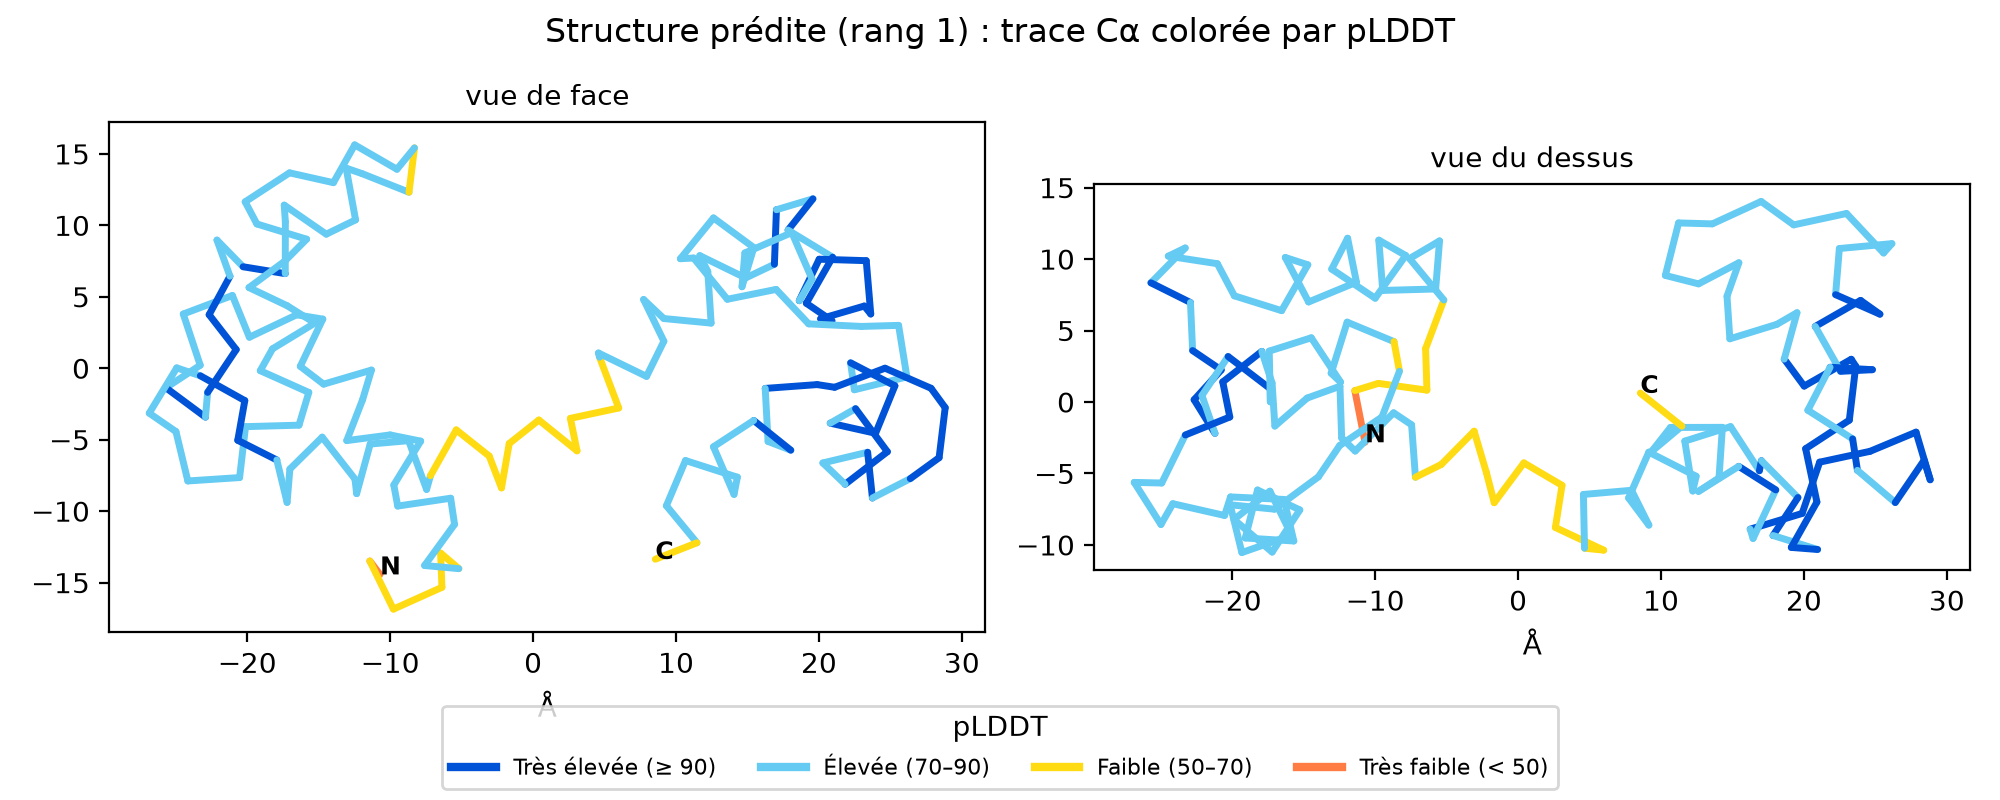
\includegraphics[width=0.95\textwidth]{../figures/P0DP23/structure.png}
  \caption{Trace C$\alpha$ du meilleur modèle, colorée par pLDDT (produite par \texttt{scripts/analyse.py}). Elle peut aussi être visualisée en 3D en déposant le fichier PDB sur \url{https://molstar.org/viewer/}.}
  \label{fig:structure}
\end{figure}

%====================================================================
\section{Analyse des scores de confiance}
\label{sec:analyse}
%====================================================================

Les deux scores se trouvent dans le fichier \texttt{*\_scores\_rank\_001\_*.json}. Le script \texttt{scripts/analyse.py} le lit avec le module \texttt{json} de Python et produit les figures ainsi qu'un résumé chiffré (\texttt{figures/P0DP23/resume.txt}). Il vérifie aussi que le pLDDT lu dans le JSON est identique à celui stocké dans la colonne B-factor du PDB (écart maximal : 0,00).

\subsection{pLDDT : confiance locale}

\paragraph{Définition.} Le pLDDT (\emph{predicted Local Distance Difference Test}) est une note de 0 à 100 attribuée à \emph{chaque résidu}. Il estime le score lDDT-C$\alpha$~\cite{mariani2013} que la prédiction obtiendrait si on la comparait à la vraie structure. Autrement dit, il indique si les distances entre ce résidu et ses voisins proches sont correctes. Ce score est \emph{local} et ne nécessite aucune superposition~\cite{jumper2021,ebi_course}.
\begin{itemize}
  \item \textbf{$>$ 90} : très fiable, squelette et chaînes latérales compris ;
  \item \textbf{70–90} : squelette fiable, chaînes latérales parfois mal placées ;
  \item \textbf{50–70} : faible confiance ;
  \item \textbf{$<$ 50} : à ne pas interpréter. C'est souvent une région intrinsèquement désordonnée, mais cela peut aussi signifier que l'information manque, par exemple un linker entre deux domaines.
\end{itemize}
Le pLDDT sert donc à décider quelles parties de la structure on peut exploiter. En revanche, un pLDDT élevé partout \emph{ne garantit pas} que les domaines sont correctement placés les uns par rapport aux autres~\cite{ebi_course}.

\begin{figure}[H]
  \centering
  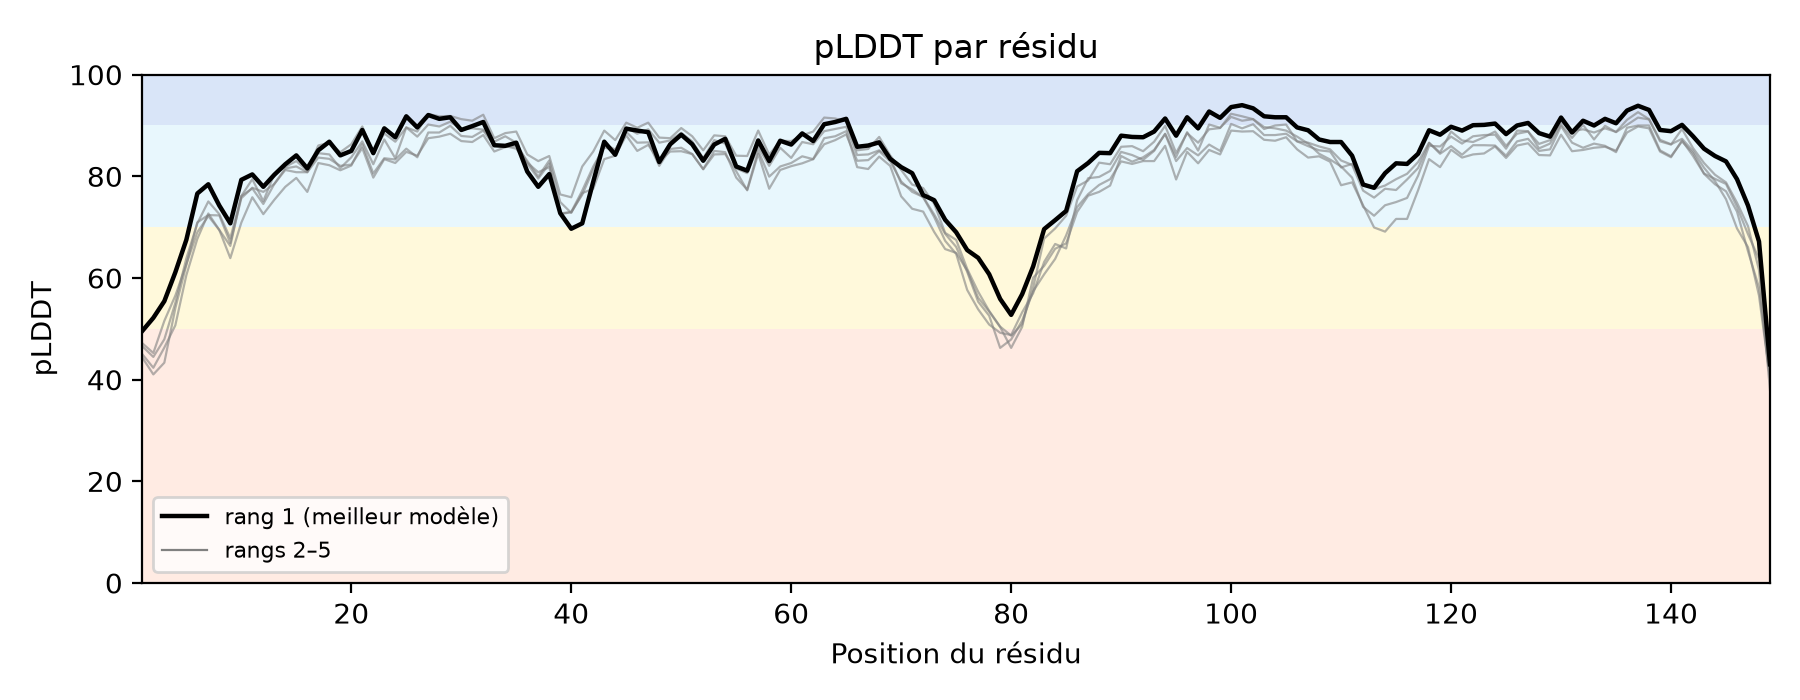
\includegraphics[width=0.95\textwidth]{../figures/P0DP23/plddt.png}
  \caption{pLDDT par résidu du meilleur modèle (noir) et des 4 autres (gris). Fonds colorés : classes de confiance.}
  \label{fig:plddt}
\end{figure}

\paragraph{Résultats.} La figure~\ref{fig:plddt} montre que 88,6~\% des résidus ont un pLDDT supérieur à 70 : 21,5~\% au-dessus de 90 et 67,1~\% entre 70 et 90. Les deux lobes (environ 6–72 et 86–145) sont prédits avec confiance, avec des maxima au-dessus de 90 dans les hélices. Trois zones descendent sous 70 :
\begin{itemize}
  \item \textbf{la région centrale 75–83} (minimum de 53 au résidu 80) : c'est le linker entre les deux lobes, dont la flexibilité en solution est connue~\cite{barbato1992} ;
  \item \textbf{les extrémités 1–5 et 148–149} (minimum de 43 au résidu C-terminal) : les extrémités libres d'une chaîne sont typiquement peu contraintes ;
  \item un léger creux vers le résidu 40, et un autre autour de 112–113 (environ 78), à la jonction entre les deux motifs EF-hand de chaque lobe.
\end{itemize}
Les 5 modèles donnent le même profil (courbes grises), ce qui montre que ces variations ne sont pas dues au hasard d'un seul modèle.

\subsection{PAE : confiance dans les positions relatives}

\paragraph{Définition.} La PAE (\emph{Predicted Aligned Error}) est une \emph{matrice} N$\times$N. La valeur (i,j) est l'erreur attendue, en ångströms, sur la position du résidu~\emph{i} si l'on superpose la prédiction et la vraie structure sur le résidu~\emph{j}~\cite{ebi_course}. Les deux axes représentent donc les résidus de la protéine : en ordonnée, le résidu dont on évalue la position ; en abscisse, le résidu sur lequel on aligne. La diagonale, qui correspond à l'alignement d'un résidu sur lui-même, vaut toujours presque zéro et ne porte pas d'information. Une valeur faible (vert foncé) signifie que la position relative des deux résidus est fiable ; une valeur élevée (vert clair) signifie qu'elle ne l'est pas.

\paragraph{Différence avec le pLDDT.} Le pLDDT répond à la question \og ce résidu est-il bien placé par rapport à ses voisins ? \fg{} ; la PAE répond à la question \og la position de ce résidu \emph{par rapport à ce résidu éloigné} est-elle fiable ? \fg{}. La PAE est donc indispensable pour juger l'\textbf{arrangement des domaines}.

\begin{figure}[H]
  \centering
  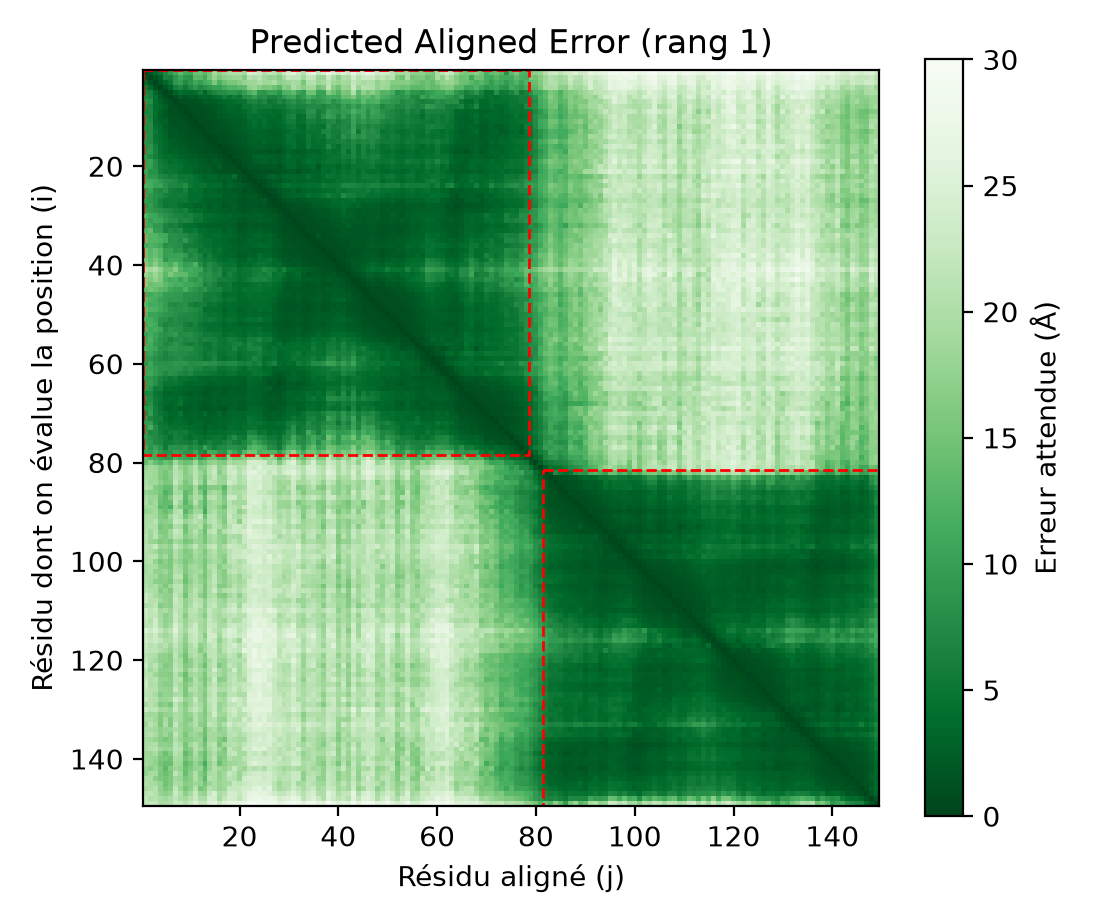
\includegraphics[width=0.55\textwidth]{../figures/P0DP23/pae.png}
  \caption{Matrice PAE du meilleur modèle. Cadres rouges : lobe N (1–78) et lobe C (82–149).}
  \label{fig:pae}
\end{figure}

\paragraph{Résultats.} La matrice (figure~\ref{fig:pae}) montre \textbf{deux blocs vert foncé} le long de la diagonale, qui correspondent aux deux lobes. La PAE moyenne vaut 5,1~Å à l'intérieur du lobe N et 3,8~Å à l'intérieur du lobe C : chaque lobe est une unité rigide bien prédite. En revanche, les \textbf{blocs hors diagonale} sont clairs, avec une PAE moyenne de 20,6 et 19,7~Å entre les deux lobes. AlphaFold2 est donc sûr de la forme de chaque lobe, mais \emph{pas} de leur orientation l'une par rapport à l'autre.

C'est l'exemple typique où le pLDDT seul induirait en erreur. Hormis le linker, presque tous les résidus ont un pLDDT supérieur à 70, et pourtant la position relative des lobes dans le fichier PDB n'est qu'une conformation parmi d'autres possibles. Ce résultat est cohérent avec le pTM modeste (0,49) et avec la flexibilité connue de la calmoduline, dont la région centrale se replie pour envelopper ses peptides cibles. Enfin, AlphaFold2 ignore les ions : la structure est prédite sans les quatre Ca$^{2+}$ qui, dans la cellule, modifient la conformation des lobes.


%====================================================================
\section{Retour d'expérience}
%====================================================================

\paragraph{Ce qui a fonctionné.} L'image Docker de ColabFold a fonctionné du premier coup sur une machine sans GPU. Le serveur MMseqs2 a construit le MSA en quelques secondes. Le point essentiel est que toute la chaîne, de la séquence à la structure puis aux figures, tient en deux commandes (\texttt{predict.sh} puis \texttt{analyse.py}), sans installation de bases de données.

\paragraph{Ce qui a posé problème.} Le temps de calcul sur CPU (\todo{durée}) est le principal inconvénient. Il devient prohibitif au-delà de quelques centaines de résidus, car le coût croît à peu près comme le carré de la longueur. Viennent ensuite des détails pratiques (droits des fichiers, noms trop longs) qui ne sont documentés nulle part de façon centralisée.

\paragraph{Recommandations.}
\begin{itemize}
  \item Sans GPU et pour une protéine de plus de 300 résidus, utiliser le notebook ColabFold sur Google Colab, qui produit exactement les mêmes fichiers ; le script d'analyse s'applique tel quel.
  \item Pour un premier essai, réduire le calcul avec \texttt{--num-models 1}.
  \item Toujours lire le pLDDT \emph{et} la PAE avant d'interpréter la structure, et ne jamais conclure sur l'orientation relative de deux domaines sans consulter la PAE.
  \item Le serveur MMseqs2 est une ressource partagée : ne pas soumettre des centaines de séquences d'un coup.
\end{itemize}

%====================================================================
\section*{Utilisation de l'IA générative}
%====================================================================

Ce projet a été réalisé avec l'aide de Claude (Anthropic), utilisé via Claude Code, pour la comparaison des solutions techniques, la mise en place de l'environnement Docker, l'écriture des scripts \texttt{predict.sh} et \texttt{analyse.py}, la rédaction du \texttt{README.md} et de ce rapport, ainsi que l'interprétation du pLDDT et de la PAE. Tous les contenus ont été relus et vérifiés, en particulier par rapport aux sources citées. Lien public vers la conversation : \todo{lien de partage de la conversation}.
